\documentclass[a4paper,10pt,openright,titlepage]{report}

\usepackage[utf8]{inputenc}
\usepackage{wasysym}
\usepackage{amsfonts}
%%\usepackage{amsmath}
\usepackage{amssymb}
\usepackage{amsthm}
\usepackage{fancyhdr}
\usepackage[french]{babel}
\usepackage{xspace}
\usepackage{lmodern}
\usepackage[babel]{microtype}
\usepackage[T1]{fontenc}
\usepackage{graphicx}

\usepackage{hyperref}
\hypersetup{%
   pdfauthor=Hauweele David%
}

\title{Synthèse physique second semestre}

\author{Hauweele David}
\date{\today}

\newtheorem{ex}{Exercice}

\newcommand{\conseq}{\rightsquigarrow}
\newcommand{\eqsyst}[2]{\left\lbrace\begin{array}{ll}#1\\#2\end{array}\right.}
\newcommand{\so}{\Rightarrow}
\newcommand{\os}{\Leftarrow}
\newcommand{\ioi}{\Leftrightarrow}
\newcommand{\tset}[1]{\left\lbrace #1 \right\rbrace}
\newcommand{\R}{\mathbb{R}}
\newcommand{\C}{\mathbb{C}}

%%Some lnalg command set :)
\newcommand{\rd}{\circ}
\newcommand{\apl}[3]{#1 : #2 \rightarrow #3 \mbox{ une application } K \mbox{-lineaire}}
\newcommand{\Apl}[2]{#1 : #2 \rightarrow #2 \mbox{ une application } K \mbox{-lineaire}}
\newcommand{\ap}{ \rightarrow }
\newcommand{\apw}[1]{\stackrel{#1}{\rightarrow}}
\newcommand{\kev}{K-\mbox{espace vectoriel }}
\newcommand{\im}{\mbox{ Im }}
\renewcommand{\ker}{\mbox{ Ker }}

%%some physical unit 
\newcommand{\Hz}{\textit{Hz}}

\begin{document}
\maketitle
\tableofcontents
\newpage

\part{Electricité et magnétisme}

\section{Charge électrique}
\subsection{Loi de coulomb}
Pour une charge sphérique :
$$F=\frac{1}{4 \pi \varepsilon_0} \frac{q_1 q_2}{r^2} \vec {1_r}$$
Valable uniquement pour des charges immobiles

\subsection{Distribution de charges}

\begin{itemize}
\item{Volumique $\rho (C/m^3)$}
\item{Surface $\sigma (C/m^2)$}
\item{Linéaire $\lambda (C/m)$}
\end{itemize}

$$\sum q = \int dq =$$
$$\int_{r_1}^{r_2} \lambda dr$$
$$\int_{a_1}^{a_2} \sigma da$$
$$\int_{v_1}^{v_2} \rho dv$$

\section{Champ électrique}
$$\vec F = q \vec E$$

Unités du champ électrique : $N/C$

\subsection{Champ sphérique}

$$\vec E = \frac{1}{4 \pi \varepsilon_0} \frac{q}{r^2} \vec {1_r}$$

Avec $q$ la charge à l'origine du champ

\subsection{Champ produit par une distribution de charge}

$$\vec E = \int d{\vec E} = \int \frac{1}{4 \pi \varepsilon_0} \frac{dq}{r^2} \vec {1_r}$$

\subsection{Dipole électrique}

$$\vec E = - \frac{1}{4 \pi \varepsilon_0} \frac{2 q a}{y^3} \vec {1_x}$$

Moment dipolaire $2qa$ , unités : $C.m$

\subsection{Flux électrique}

$$\Phi_E = \vec {E}.\vec A$$
$$\Phi_E = \sum \Phi_{E_i} = \oiint \vec E.d \vec A$$

Unités du flux électrique : $N.m^2 / C$

\section{Théorème de Gauss}

$$\oint \vec E d \vec A = \frac{q_i}{\varepsilon_0}$$

\subsection{Symétrie}

\begin{itemize}
\item{Symétrie axiale cylindrique : $\vec E = \frac{\lambda}{2 \pi r \varepsilon_0}$}
\item{Symétrie plane : $\vec E = \frac{\sigma}{2 \varepsilon_0}$}
\end{itemize}


\section{Matière dans un champ électrique}
\subsection{Charge dans un champ électrique}
$$a = \frac{q}{m} E$$
\subsection{Equilibre électrostatique}
A l'équilibre électrostatique, le champ dans un conducteur est toujours nul indépendamment de la forme du conducteur, du champ appliqué, de la nature du conducteur.

\begin{figure}[!h]
\centering
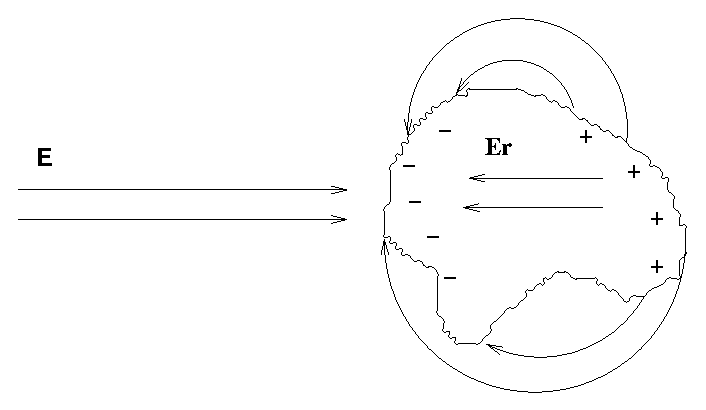
\includegraphics{eqelec.eps}
\caption{Illustration de l'équilibre électrostatique}
\end{figure}

Dans un conducteur il n'y a pas de champ électrique et les charges en excés sont sur sa surface.

\subsection{Champ électrique à la surface d'un conducteur chargé}
$$E = \frac{\sigma}{\varepsilon_0}$$

\subsection{Dipole dans un champ électrique}
$$U = -p.E$$

Avec $p$ le moment dipolaire

\subsection{Dipole dans un champ électrique non homogène}

$$F=(p.\nabla)E$$

\section{Potentiel électrostatique}
$$\Delta V = \frac{W_{AB}}{q} = - \int_A^B E.dl$$

Unité de la différence de potentiel : volt ($V$)

$$\vec \nabla V = - \vec E$$

$$\vec \nabla . \vec E = \frac{\rho}{\varepsilon_0}$$

$$\nabla^2 V = - \frac{\rho}{\varepsilon_0}$$

$$V(r) = \frac{q}{4 \pi r \varepsilon_0} \mbox{ pour une charge ponctuelle}$$

\section{Energie électrique}

\subsection{Energie d'un système de charges ponctuelles}

$$U(r) = q_1 V_2(r) = q_2 V_1(r)= \frac{q_1 q_2}{4 \pi r \varepsilon_0}$$

$$U = \frac{Q_1 V_1}{2}+ \frac{Q_2 V_2}{2} + \ldots + \frac{Q_n V_n}{2}$$

\subsection{Energie électrique de deux grandes plaques}

Energie de deux grandes plaques métalliques de surface $A$ et séparées par une distance $d$. Des charges $+Q$ et $-Q$ sont respectivement placées sur ces plaques. 

$$U = \frac{\varepsilon_0 E^2}{2} . \mbox{ volume ou se trouve le champ }$$

\subsection{Densité d'énergie}

$$U=\int \frac{\varepsilon_0 E^2}{2} dv$$

\section{Condensateurs et diélectriques}

$$Q=CV$$
$$C=\frac{Q}{V}$$
$$C=\frac{Q}{\Delta V}$$

Unité de capacitance : Farad ($F = C^2/{N.m}$)

\subsection{Capacitance de la sphère}

$$C=4 \pi \varepsilon_0 r$$

\subsection{Capacitance d'un condensateur (double plaque)}

Un condensateur formé par deux plaques de surface $A$ séparées d'une distance $d$.

$$C = \frac{\varepsilon_0 A}{d}$$

\subsection{Condensateurs en série}

$$C = \left( \sum_i \frac{1}{C_i} \right)^{-1}$$

\subsection{Condensateurs en parallèle}

$$C = \sum_i C_i$$

\subsection{Diélectriques}

$$\Delta V = \frac{\Delta V_0}{k}$$
$$C = k C_0$$

\section{Courant électrique, loi d'Ohm}

\subsection{Courant électrique}

$$I = \frac{dq}{dt}$$

Unité du courant : Ampère ($A = C/s$)

\subsection{Densité du courant}

$$\vec j = \frac{dI}{d {\vec A}}$$
$$I = \int \vec j.d\vec A$$

\subsection{Resistivité}

$$\rho = \frac{\Delta V}{E}$$

Unité de résistivité : $\Omega.m$

\subsection{Loi d'ohm}

$$\Delta V = R I$$
$$j=\frac{E}{\rho}$$

Unité de résistance : Ohm ($\Omega$)

\subsection{Loi de Pouillet}

Avec un conducteur de longeur $l$ et de résistivité $\rho$ de section $A$

$$R = \frac{\rho l}{A}$$

\subsection{Résistance en série}

$$R = \sum_i R_i$$

\subsection{Résistance en parallèle}

$$R = \left( \sum_i \frac{1}{R_i} \right)^{-1}$$

\section{Force magnétique et champ magnétique}

\subsection{Force magnétique}

$$\vec F = \frac{\mu_0 q_1 q_2}{4 \pi r^2} \vec v_1 \times (\vec v_2 \times \vec 1_r)$$

\subsection{Champ magnétique}

Une charge $q$ à une vitesse $\vec v$ dans un champ $\vec B$.

$$\vec F = q \vec v \times \vec B$$

$$\vec B = \frac{\mu_0 q}{4 \pi r^2}(\vec v \times \vec {1_r}$$

Si $\vec v$ perpendiculaire à $\vec B$ alors $B = \frac{F}{qv}$

Unité de champ magnétique : Tesla ($T = N/(C.m/s) = Wb/m^2$)

Autre unité de champ magnétique : Gauss ($G = 10^{-4} T$)

\subsection{Flux magnétique}
$$\Phi_B = \oint \vec B.d \vec A$$

Unité de flux magnétique : Weber ($Wb = T.m^2$)

\subsection{Loi de Gauss pour un champ magnétique}

$$\oint \vec B . d\vec A = 0$$

\subsection{Loi de Biot - Savart}

$$dB = \frac{\mu_0}{4 \pi} \frac{I d \vec l \times \vec {1_r}}{r^2}$$

\subsection{Champ magnétique d'un fil long et fin et courant constant}

Le champ magnétique à une distance $d$ perpendiculairement au fil

$$B = \frac{\mu_0 I}{2 \pi d}$$

\section{Loi d'Ampère}

$$\oint \vec B . d \vec l = \mu_0 I$$

\subsection{Champ magnétique d'un fil long de section $s$}

\subsubsection{A l'intérieur}
$$B=\frac{\mu_0 I_0 r}{2 \pi s^2}$$

\subsubsection{A l'extérieur}
$$B=\frac{\mu_0 I_0}{2 \pi r}$$

\subsection{Solénoïde}

\begin{figure}[!h]
\centering
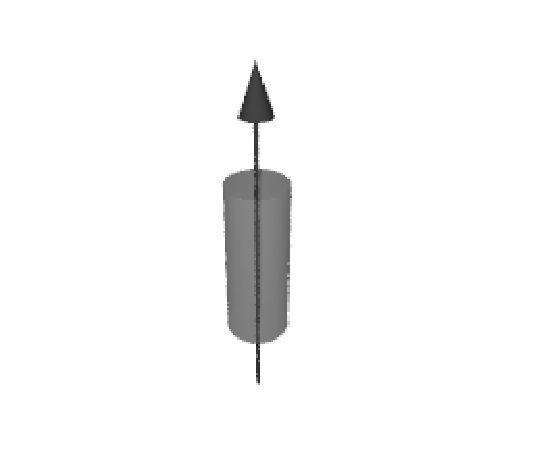
\includegraphics{solenoide.eps}
\caption{Champ magnétique dans un solénoïde}
\end{figure}

$$B = \mu_0 I_0 n$$

\newpage

\subsection{Toroïde}

\begin{figure}[!h]
\centering
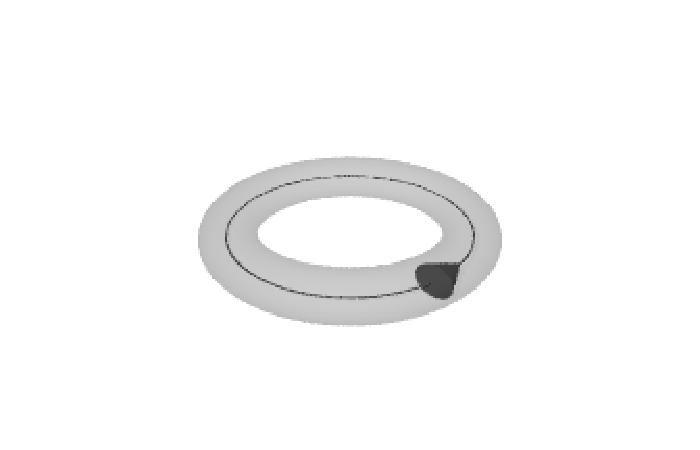
\includegraphics{toroide.eps}
\caption{Champ magnétique dans un toroïde}
\end{figure}

$$B = \frac{\mu_0 N I_0}{2 \pi r}$$

\subsection{Force de Lorentz}

$$F= qE + qv \times B$$

\section{Induction}

\subsection{Force électromotrice induite}

C'est la différence de potentiel induite

$$\varepsilon = - \frac{d \Phi_B}{dt}$$ 

\subsection{Champ électrique induit}

On a $E'$ le champ électrique induit, non conservatif.

$$\varepsilon = \int E' dl$$

$$\oint E'.dl = -\frac{d\Phi_B}{dt}$$

\subsection{Inductance}

$$\Phi_B = L I$$
$$\varepsilon = - L \frac{dI}{dt}$$

Unité d'inductance : Henry ($H = V.s/A$)

\subsection{Energie magnétique}

$$U = \frac{LI^2}{2}$$

\subsection{Densité d'énergie magnétique dans un solénoïde}

$$u_B = \frac{B^2}{2 \mu_0}$$

\section{Constante}
\subsection{Constante de permitivité}
$$\varepsilon_0 = 8,85.10^{-12} C^2/(Nm^2) \mbox{ ou } F/m$$

\subsection{Constante de perméabilité}
$$\mu_0 = 4 \pi 10^{-7} \frac{N.s^2}{c^2} = 1,26.10^{-6} \frac{N.s^2}{c^2} \mbox{ ou }H/m$$

\subsection{Capacitance de la terre}
$$C_{\mbox{terre}} = 7,1.10^{-4} F$$

\part{Ondes}

\section{Généralités sur les ondes}
\subsection{Equation d'onde à une dimension}
La fonction $\Gamma(x,t) = \gamma(x - v t) $ est une onde ssi elle vérifie la propriété suivante :
$$\frac{\partial^2 \Gamma}{\partial t^2} = v^2 \frac{\partial^2 \Gamma}{\partial x^2}$$
Avec $\gamma$ la valeur de l'onde en $x$ et $\Gamma$ la fonction d'onde et $v$ la vitesse de propagation de cette onde.
\subsection{Ondes harmoniques}
Forme générale d'une onde harmonique:
$$y(x,t) = A \sin (k x - \omega t) + B \sin (k x + \omega t)$$

\begin{itemize}
 \item{nombre d'onde $k$ (unit. $m^{-1}$)}
 \item{longeur d'onde $\lambda$ (unit. $m$)}
 \item{pulsation ou fréquence angulaire $\omega$ (unit. $s^{-1}$)}
 \item{période $T$ (unit. $s$)}
 \item{fréquence $\nu$ (unit. $\Hz$)}
 \item{vitesse de phase de l'onde $v$ (unit. $m/s$)}
\end{itemize}
\begin{center}
% use packages: array
\begin{tabular}{|l|}\hline
$\lambda = 2\pi/k$\\ \hline
$\omega = 2\pi/T$ \\ \hline
$\nu = 1/T$ \\ \hline
$v = \nu \lambda =\omega/k$ \\ \hline
\end{tabular}
\end{center}

\subsection{Vitesse des ondes dans un fil}
$$v = \sqrt{\frac{T}{\mu}}$$
Avec $T$ la tension du fil et $\mu$ la densité du fil ($kg/m$).

\subsection{Energie d'une onde transverse dans un fil}
$$dU = \frac{1}{2} T \left(\frac{dy}{dx} \right)^2 dx$$
$$dE = dE_{cin}+dU = \frac{dx}{2} \left[\mu \left( \frac{\partial y}{\partial t}\right)^2 + T \left( \frac{\partial y}{\partial x}\right)^2 \right]$$
$$\frac{dE}{dx} = \frac{1}{2} \left[ \mu \left( \frac{\partial y}{\partial t}\right)^2 + T \left( \frac{\partial y}{\partial x}\right)^2 \right]$$
\subsubsection{Application aux ondes harmoniques}
$$\frac{dE}{dx} = \mu \omega^2 A^2 \sin^2 (kx - \omega t)$$
$$P = \frac{dE}{dt} = v\frac{dE}{dx} = v\mu \omega^2 A^2 \sin^2(kx-\omega t)$$
\subsection{Principe de superposition}
$$A \cos(k_1 x - \omega_1 t) + A \cos(k_2 x - \omega_2 t) = 2A \cos \left( \frac{\Delta k - \Delta \omega t}{2} \right).\cos \left( \frac{\Sigma k - \Sigma \omega t}{2} \right)$$
$$\nu_{\mbox{battement}} = \nu_1 - \nu_2$$
\subsection{Ondes stationnaires}
$$A \cos (kx - \omega t) + A \cos(kx + \omega t) = 2A \cos (kx) . \cos (\omega t)$$

Fréquence propre :

$$\nu_n = \frac{n v}{2L}$$

Longueur d'onde :

$$\lambda_n = \frac{2 L}{n}$$

Nombre de noeuds :

$$N = n + 1$$

\begin{center}
% use packages: array
\begin{tabular}{|l|l|l|}\hline
\bfseries Mode normal ($n$) & \bfseries Noeuds ($N$) & \bfseries Nom \\ \hline
1 & 2 & Fondamental \\ \hline
2 & 3 & 1 harmonique \\ \hline
3 & 4 & 2 harmonique \\ \hline
4 & 5 & 3 harmonique \\ \hline
5 & 6 & 4 harmonique \\ \hline
\end{tabular}
\end{center}

\section{Ondes electromagnétiques}
\subsection{Equation d'onde électromagnétique}
$$\frac{\partial^2 E}{\partial t^2} = \sqrt{c}\frac{\partial^2 E}{\partial x^2}$$
$$E = E(x-ct)$$
$$\frac{\partial^2 B}{\partial t^2} = \sqrt{c}\frac{\partial^2 B}{\partial x^2}$$
$$B = B(x-ct)$$
$$E=cB$$
\subsection{Solution de l'équation d'onde électromagnétique}

\begin{center}
% use packages: array
\begin{tabular}{ll}
$E_y (x,t) = E_0 \sin(kx - \omega t)$ & $E_z (x,t) = \pm E_0 \sin(kx - \omega t)$ \\ 
$B_z (x,t) = \pm B_0 \sin(kx - \omega t)$ & $B_z (x,t) = B_0 \sin(kx - \omega t)$
\end{tabular}
\end{center}

$$E = \sqrt{E^2_y + E^2_z} = E_0$$
$$B = \sqrt{B^2_y + B^2_z} = B_0$$

Les ondes électromagnétiques planes sont transversales, les champs $E$ et $B$ sont perpendiculaires entre eux et à la direction de propagation.
\subsection{Energie et impulsion d'une onde électromagnétique}

Densité d'énergie associée à un champ électrique : 

$$E_E = 1/2 \epsilon_0 E^2$$

Densité d'énergie associée à un champ magnétique :

$$E_B = 1/(2\mu_0) B^2 = 1/(2\mu_0) c^2 E^2 = 1/2 \epsilon_0 E^2 = E_E$$

Densité totale d'énergie :

$$E_{\mbox{tot}} = \epsilon_0 E^2$$

Intensité de l'onde (énergie par unité de temps à travers une surface) :

$$I = E_{\mbox{tot}} c = c \epsilon_0 E^2$$
$$I_{\mbox{moyen}} = \frac{c \epsilon_0 E^2_0}{2}$$

\subsubsection{Vecteur de Poynting}
Le vecteur de Poynting est définie par :

$$\vec P = \vec S = \frac{1}{\mu_0} \vec E \times \vec B$$

Son module vaut l'intensité instantanée $I$ de l'onde.
\subsubsection{Impulsion}
L'impulsion d'une onde électromagnétique est donnée par :

$$p = E_{\mbox{tot}}/c = \epsilon_0 E/c = \epsilon_0 (\vec E \times \vec B)$$

$$\oint P dS = \frac{dE}{dt}$$
\subsubsection{Moment cinétique}
Le moment cinétique d'une onde électromagnétique est donné par :

$$L = r \times p = \epsilon_0 r. (\vec E \times \vec B)$$

Une particule qui émet ou absorbe une onde électromagnétique modifie son énergie et sa quantité de mouvement mais aussi son moment cinétique.

\subsection{Pression de radiation}

Pression produite par une radiation tombant sur une surface $A$ et normale à celle-ci.

$$P_n = \alpha (1+\rho) E_{\mbox{tot}}$$

Avec $\alpha = 1$ si la radiation tombe perpendiculairement par rapport à la surface, $\alpha = 1/3$ si la radiation vient dans toutes les directions par rapport à la surface.

Avec $\rho$ la capacité du corps à absorber les ondes 0 (absorbe totalement, corps noir) à 1 (totalement réfléchissant).

\section{Interférences}

\subsection{Ondes électromagnétiques stationnaires}
$$E_0 cos (\omega t - \omega x /c) - E_0 cos ( \omega t + \omega x/c ) = 2 E_0 \sin (\omega t).\sin(\omega x/c)$$


Les maxima pour $E$ se trouvent en $x = \frac{(1+2n)\lambda}{4}$.\\

Les noeuds pour $E$ se trouvent en $x = \frac{n \lambda}{2}$.\\

Les maxima pour $B$ se trouvent en $x = \frac{n \lambda}{2}$.\\

Les noeuds pour $B$ se trouvent en $x = \frac{(1+2n)\lambda}{4}$.

\subsection{Les films minces}

Soit un film mince (d'huile par exemple) de longeur $d$.\\

On a des interférences constructives quand $d = \frac{k \lambda}{2}$.\\

On a des interférences destructives quand $d = \frac{(1+2k)\lambda}{4}$.

Remarque : $\lambda$ est ici la longueur d'onde dans le film, si son indice de réfraction est $n$, ce sera $n \lambda$ dans l'air.

\subsection{Interférence par deux fentes (expériences de Young)}

On a un maximum d'intensité quand $d \sin \theta = n \lambda$.\\

On a un minimum d'intensité quand $d \sin \theta = \frac{(2n+1)\lambda}{2}$\\

Avec $d$ la distance entre les deux fentes.

$$E=E_1+E_2 = 2 A / r_0 \cos ( \omega t - \omega r_0 / c) \cos \left[ (\omega d / 2 c) \sin \theta \right]$$

Variation de l'intensité avec $\theta$ pour un écran à une distance fixe $r_0$ des fentes (donc circulaire, mais si $r_0$ est très grand un écran plat est une bonne approximation pour autant que l'oservation se limite à un petit domaine de $\theta$) :\\

Intensité $\div \frac{1}{r_0^2} \cos^2 \left( \frac{\pi d}{\lambda} \sin \theta \right)$.

\subsection{Interférence par plusieurs fentes (réseau)}

On a un maximum d'intensité quand $d \sin \theta = n \lambda$ avec $n = 0,1,2$.\\

On a un minimum d'intensité quand $d \sin \theta =\frac{m \lambda }{N}$ avec $m=1,2,3$ avec $m = N, 2N...$ exclus.\\

Pouvoir de résolution du réseau : $\frac{\lambda}{\Delta \lambda} = N n$.\\

$$\Delta \theta = \frac{\lambda}{N d}$$

\section{Diffraction}
\subsection{Diffraction par une fente simple}
Soit une onde plane frappant une fente (dont l'ordre de grandeur de la largeur est de lo'ordre de celle de longueur d'onde). Pour calculer la distribution de lumière au delà de la fente on utilise le Principe d'Huygens-Fresnel : on considère que chaque point de la fente atteint par le front d'onde peut être considéré comme la source d'une onde sphérique; l'onde totale dans la région au-delà de la fente est la supertposition de toutes ces ondes.\\

Condition pour avoir des minimas : $a \sin \theta = n \lambda$ avec $a$ la largeur de la fente.\\

Les maximas se trouve au milieu ($\theta = 0$) et entre les minimas.\\

Largeur du maxima central $\theta = \arcsin (\lambda / a)$.\\

Intensité $\div \frac{1}{r_0^2} \frac{\sin^2 \left[ \frac{\pi a}{\lambda} \sin \theta \right]}{\sin^2 \theta}$

\subsection{Diffraction par une ouverture circulaire, critère de Rayleigh}

Position angulaire du premier minima : $\sin \theta = 1,22 \lambda / a$.

Critère de Rayleigh :

$$\Delta \theta = 1,22 \lambda / a$$

\end{document}
